\documentclass[beamer]{standalone}

\usepackage{tikz}

\usetikzlibrary{backgrounds}
\usetikzlibrary{calc}
\usetikzlibrary{fit}
\usetikzlibrary{shapes.symbols}
\usetikzlibrary{positioning}

\definecolor{x-red}{HTML}{e41a1c}
\definecolor{x-blue}{HTML}{3694E0}
\definecolor{x-green}{HTML}{63E05F}
\definecolor{x-purple}{HTML}{D365E3}
\definecolor{x-orange}{HTML}{E8A100}
\definecolor{x-yellow}{HTML}{fff200}

\definecolor{almost-white}{HTML}{fefefe}

\begin{document}

\begin{standaloneframe}

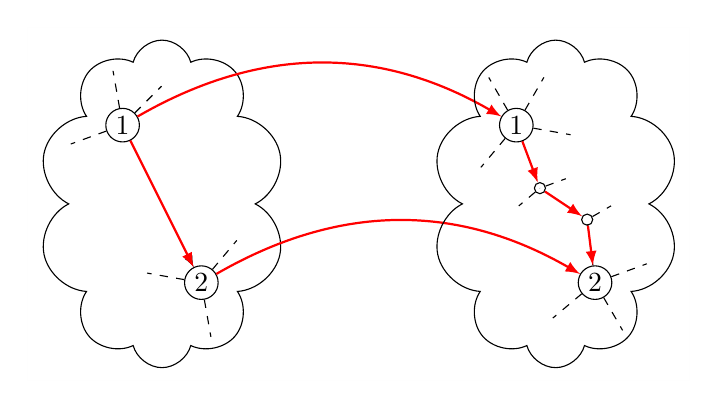
\begin{tikzpicture}[
    node/.style={draw, circle,
        inner sep=.05cm,
    },
    wire/.style={-latex},
    background rectangle/.style={ draw=almost-white, line width=0pt, },
    show background rectangle,
]

\node [node] (a) at (0,2) {\(1\)};
\node [node] (b) at (1,0) {\(2\)};

\node [cloud, cloud ignores aspect, draw, fit=(a) (b)] {};

\draw [wire] (a) to node [coordinate] (ab) {} (b);

\draw [dashed] (a) to ++(100:.7);
\draw [dashed] (a) to ++(45:.7);
\draw [dashed] (a) to ++(200:.7);

\draw [dashed] (b) to ++(280:.7);
\draw [dashed] (b) to ++(50:.7);
\draw [dashed] (b) to ++(170:.7);


% target graph

\onslide<2->{
    \node [node] (ia) at (5,2) {\(1\)};
    \node [node] (ib) at (6,0) {\(2\)};

    \draw [dashed] (ia) to ++(60:.7);
    \draw [dashed] (ia) to ++(120:.7);
    \draw [dashed] (ia) to ++(230:.7);
    \draw [dashed] (ia) to ++(350:.7);

    \draw [dashed] (ib) to ++(220:.7);
    \draw [dashed] (ib) to ++(20:.7);
    \draw [dashed] (ib) to ++(300:.7);
}

\onslide<2>{
    \node [coordinate] (ix-inv) at (5.3,1.2) {};
    \node [coordinate] (iy-inv) at (5.9,0.8) {};
    \draw [dashed] (ia) to (ix-inv);
    \draw [dashed] (ib) to (iy-inv);

    \draw [wire, red, thick] [bend left] (a) to (ia);
    \draw [wire, red, thick] [bend left] (b) to (ib);
}
\node [cloud, cloud ignores aspect, draw, fit=(ia) (ib)] {};
\onslide<3->{
    \node [node] (ix) at (5.3,1.2) {};
    \node [node] (iy) at (5.9,0.8) {};

    \draw [wire, red, thick] (a) to node [coordinate] (ab) {} (b);

    \draw [wire, red, thick] (ia) to (ix);
    \draw [wire, red, thick] (ix) to node [coordinate] (ixy) {} (iy);
    \draw [wire, red, thick] (iy) to (ib);

    \draw [dashed] (ix) to ++(220:.35);
    \draw [dashed] (ix) to ++(20:.35);
    \draw [dashed] (iy) to ++(30:.35);
}







\end{tikzpicture}


\end{standaloneframe}

\end{document}
